\chapter{Evaluation\label{cha:evaluation}}
%10041
Throughout this thesis the requirements, design and prototype implementation of
the \ep~system that can support \LLLs has been discussed. This chapter focuses
on the evaluation of this research and its contributions based on three studies.
The studies were designed to look into the specific aspects of \LLLs support and
understand how well developed features satisfy the requirements identified
earlier by the lecturers and students. 

The number of studies represents perspectives of all of the stakeholders that
have been involved in this research earlier, i.e., lecturers and students.
Reason for this was to ensure that all of the perspectives are being captured as
\textit{different stakeholders often have different perspectives}
\citep[p.~111]{Hevner2010}. In addition, the evaluation from the students'
perspective has been split into two studies as the requirements elicitation
stage discovered that the perception of \LLLs depends on the maturity of
students. Therefore, it was decided to use different evaluation approaches for
each group of students.

The first section of this chapter describes the approaches and data collection
methods used in the evaluation stage. Further, each of the three studies is
presented with the detailed participants profile description, exercise protocol
followed by the study, artifacts collected and the results of data analysis.
Each study section ends with conclusions that look into recommended improvements
to the \ep~system prototype and its processes.

\section{Design Overview}
As this chapter aims to evaluate this research and its contributions, the
relevant research question and its sub-questions are restated here:

\textit{How does the extended environment meet the needs of the stakeholders in
university teaching and learning contexts?}
\textit{\begin{itemize}
  \item How can lecturers use new features to provide students with their
  guidance and help them to understand \LLLs skills?
  \item How can students address \LLLs skills using new features?
  \item How can new features help students track their learning progress, manage
  \ep~knowledge and organize content, demonstrate and share their
  achievements with others?
\end{itemize}}

To answer these questions, three studies were carried out independently from
each other. The results were used to evaluate the developed prototype from three
different perspectives: lecturers, mature students and less experienced
students. Each study followed its own exercise protocol described in the related
sections. Detailed design of each study can be found further in this chapter in
Sections \ref{sec:one}, \ref{sec:two}, and \ref{sec:three} respectively.

Data collection for analysis was performed using both quantitative and
qualitative methods to support the principles of multiple sources and multiple
perspectives of data advocated by many researchers
\citep{Yin2009,Maimbo2005,Marshall2010}. The following techniques were used over
the course of all studies:

\begin{itemize}
  \item Behavior observations made by the researcher during all studies.
  \item Observation data in form of digital photographs taken during the group
  experiments.
  \item Audio recordings of the face-to-face interviews collected to facilitate
  more thorough interview analysis.
  \item Open-ended questions asking for participants opinion on the features and
  tools used in the studies.
  \item Close-ended questions that required participants' evaluation based on
  ten point scale, from \textit{not useful at all} to \textit{highly useful}, 
  included in exit questionnaire.
  \item Physical artifacts in form of paper records made by participants of the
  group experiment.
  \item Digital artifacts in form of electronic records in the \ep~system made
  by participants of the group experiment and case studies.
  \item System logs demonstrating \ep~system use by case study participants.
  \item Additional evidence, comments and opinions collected by the researcher
  through informal discussions that would help to support analysis and
  conclusions.
\end{itemize}

Audio recordings as well as digital photographs were collected with the
permission of the participants and performed without interrupting the process of
each study. More detailed description of data collection methods for each study
can be found in the relevant sections this chapter and associated appendices. 

\section{Ethical Considerations}

Similarly to the earlier stage of the requirements elicitation, the Massey
University Ethics Approval process was followed for the evaluation studies of
this research. Analysis of the evaluation design with the Human Ethics Chair
concluded that none of the three studies required full ethical approval.
Therefore, a ``Low Risk Notification" was submitted to the Massey University's
Low Risk Database.

Ethics documentation, such as the Ethics Approval Letter, lecturers and students
information sheets and participants' consent forms, used for this research
stage, can be found in Appendix \ref{cha:app5}.

\section{Study One. Exploratory Evaluation by Lecturers}
\label{sec:one}

To achieve the ultimate goal of this research project to develop a system that
can provide support for \LLLs in universities, it is important that learning
facilitators, e.g. lecturers, could successfully utilize improved technology to
help and guide students in their learning journey. Therefore, this study
explores the prototype implementations from the lecturers' perspective to
understand whether their initial requirements were met.

\subsection{Goals}

The goal for this study was:

\smallquote{To find out whether lecturers can use new features to provide
students with their guidance and support, and help them to understand \LLLs
skills.}

To support achievement of this goal, the main objectives were:

\begin{itemize}
  \item To evaluate whether new features can provide better communication
  opportunities between lecturers and students;
  \item To determine how lecturers can use new features to help students
  understand the link between \LLLs skills and their university degree study;
  \item To explore how lecturers can utilize new features in the classroom to
  guide students through development of \LLLs skills. 
\end{itemize}

\subsection{Research Protocol}

This study was an exploratory study that used a demonstration and participants
interviews as a research evaluation approach. According to \citet{Peffers2008},
\textit{demonstration} is normally used to show that idea works and precedes a
more \textit{formal} evaluation. In this research project, demonstration was
included into the overall evaluation design. The expectation was that in
combination with the participant interviews, followed after each demonstration,
it would provide a valuable insight into the lecturers' perspective on the
prototype features.

For the purpose of this study, six one-on-one interviews and one small group
discussion were organized with the participants. Group discussion was undertaken
during the annual staff meeting and involved three participants.

This study did not follow a strictly defined research protocol as the directions
of the meeting discussions were based on the outcomes of the semi-structured
conversations with the participants. Each meeting started with the brief
introduction of the research and the purpose of the demonstrations undertaken.
To guide the course of the study, the researcher initially had a set of topics
to cover in the presentation and demonstrate the prototype functionality with
the examples of how it could be potentially adopted in the learning environment.
The discussion topics were based on the implemented features described in detail
earlier in Chapter \ref{cha:prototype}.

Each of the topics was presented to the participants in the following order:

\begin{itemize}
  \item the problem addressed in the topic;
  \item an implementation suggested to solve the problem;
  \item a step-by-step demonstration of how this implementation works in the
  \ep~system;
  \item expected/intended use of the feature in the classroom;
  \item where possible, examples of use in the \ep~system.
\end{itemize}

After the demonstrations, the participants were asked to assess the prototype
features based on their personal and professional experience. From their
perspective they evaluated whether the presented scenarios of use were realistic
and what challenges they could see in the suggested ways of using the features.

The lecturers were then asked to suggest how they would use new features and how
they would apply the methods these features incorporate with their students. At
the end of the topic discussion, the participants were offered to recommend the
potential improvements.

All interviews were audio recorded and transcribed for the purpose of more
thorough analysis. Direct citations in the results section (Section
\ref{sec:study1results}) were taken from the interviews transcripts.

\subsection{Participants Profile}

This study used a number of techniques to identify suitable participants.
Initially, each of the lecturer-participants of the previous stage of
identifying requirements for \LLLs supported by \ep~systems was offered to take
part in the evaluation of the prototype implementations at the later stages of
this research. Three lecturers expressed interest in continuing their
participation in the project.

The rest of the participants were recruited using snowball sampling strategy
which had already been employed earlier in this research. This strategy relied on
recommendations of the existing participants having knowledge of the suitable
candidates who would potentially be interested in this research. Based on
criteria of being a lecturer or having previous lecturing experience, and
also having experience of using an \ep~system with the students, six other
participant were identified from the suggested candidates.

Overall, the data was gathered from nine participants, all lecturers at
various schools and colleges of Massey University. Table \ref{tab:study1part}
shows demographics of the participants:

\begin{table}[htb]
  \begin{center}
    \begin{tabular}{| l | c |}
    \hline
     \multicolumn{1}{|c|}{\textbf{University Structure}} &
     \multicolumn{1}{c|}{\textbf{Number}} \\ \hline
		College of Science: & \\ 
		-- School of Engineering and Advanced Technology & 1 \\
		-- Institute of Veterinary, Animal and Biomedical Sciences & 1 \\
		-- Institute of Food, Nutrition and Human Health & 1 \\ \hline
		College of Education: & \\ 
		-- School of Curriculum and Pedagogy & 2 \\
		-- School of Educational Studies &  3 \\ \hline
		Centre for Teaching and Learning & 1 \\ \hline
	\end{tabular}
  \end{center}
\caption{Demographics of the Study One participants (n = 9)}
\label{tab:study1part}
\end{table}

One of the participants was a program coordinator for a Bachelor degree program
and had a particular interested in how the prototype functionality can be used
with the university graduate attributes and \LLLs skills.

The lecturers from the College of Education had the most experience of using
portfolios or \ep s with their students. The reason for this was that every
potential teacher in New Zealand had to meet the requirements developed by the
New Zealand Teachers Council in form of Graduating Teacher
Standards\footnote{\url{http://www.teacherscouncil.govt.nz/te/gts/}}. These
standards closely resemble university graduate attributes and \LLLs skills.
Teaching portfolio has to be created by students as a proof that they meet these
standards. The College of Education lecturers were at the earlier stages of
adoption of the institutionally supported \ep~system for these purposes and
therefore were highly interested in giving their feedback on the prototype
implementations.

A representative of the Centre for Teaching and Learning was considered a
suitable participants as they had previous teaching experience, both at school
and at university, and at that time was assisting adoption of the new learning
technologies, \ep~systems in particular, in the university courses.

Each participant was approached by an invitation email to take part in this
research and evaluate the developed features in a face-to-face meeting with the
researcher.

\subsection{Results}
\label{sec:study1results}

In general, feedback given by the lecturers based on the demonstrations was
positive.

Concept mapping \ep~module with all adjacent to it features such as
artifact's fragment extraction, timeline progress tracking and sharing
opportunities raised the most interest among the lecturers.

Some lecturers looked that the demonstrated features from the assessment
perspective. Version control in the \ep~system was found useful for giving
better feedback to student and tracking their responses as well as progress.
Concept maps was called a tool for more rigorous assessment of students'
understanding of the concepts they have learnt. Some of the lecturers had been
using mapping techniques for assessment of their students' knowledge before and
said that having the tools that could support concept mapping in the \ep~system
would be very useful.

From another perspective, as it was described by the lecturers, students might
be interested in using the new concept mapping tools for two reasons: to
communicate what they have learnt to somebody else or to try to make sense of
the things that they are learning at the moment.

One lecturer said that they liked concept mapping module in particular for its
potential to provide support for both horizontal and vertical integration of
knowledge and skills. Integrating the knowledge of their study degree as well as 
bringing together the things that students learn from other subjects is very
important:

\shortquote{What I like about this tool is that at the end students should be
able to clearly see how everything is built towards them achieving these
[graduate] attributes or not.}

However, stepping away from discussion of implementations, another participant
noticed that the problem with the new tools might be that students are less
likely to use them \textit{``for their own good''}. Therefore, an element of
assessment might be required at first. In this case, it becomes an exercise that
needs to be completed which is not the same thing as using system on learner's
own motivation.

Two of the participants mentioned that, before making any serious decision
whether the demonstrated features are feasible for use with students, they would
like to hear their opinion on these features:

\shortquote{I can see some opportunities for what we are trying to do in the
future. I definitely see potential. However, to be sure, I would be interested
in the students try to use these tools and tell us how they see it.}

The group meeting with three lecturers from College of Education had the most
active discussion of the implementations compared to one-on-one interviews
with other participants. These lecturers just finished their first trial with
the students where they were using an institutional \ep~system for creating
students' teaching profile. As a result, they had most recent experience with
students using an \ep~system to support \LLLsn.

According to the feedback given, the following are the attributes of the
implementations that the participants of the group meeting liked most of all:

\begin{itemize}
  \item Visual nature of concept mapping;
  \item Simplicity of making complex things;
  \item Challenge of conceptual understanding;
  \item Authentic evidence that students meet the outcomes;
  \item Opportunity for various levels of feedback;
  \item Ability to draw attention to the specific elements with fragment
  extraction;
  \item Ability to see students' progress towards learning goals.
\end{itemize}

Along with the positive features, a number of potential challenges were noted:

\begin{itemize}
  \item Not only students, but lecturers as well require training on how to
  use new systems and new features in their classroom:
  \shortquote{Teachers need training too. We used to think that teachers know
  everything and know how to bring new technology to their classroom. But in
  reality, they don't.}
  
  \item Students need assistance throughout the process of learning the
  \ep~system: 
  \shortquote{We have all sorts of students and not all of them are on good
  terms with technology. Some struggle with such simple things as writing a
  blog or creating a web page, even when they have all the instructions
  required. If you want this system to be accepted by students, they need to be
  sure that help is always out there for them.}
  
  \item Curriculum should be adjusted to support \LLLsn:
  \shortquote{Our challenge is to develop the notion of \LLLs ability and what
  it means for that to be a good practicing [engineer, lawyer, doctor]. And we
  need to embed it early on, because they [students] don't know the notion at
  the moment.}
\end{itemize}

It is also important to mention that after the formal part, five out of nine
participants asked when they could expect to see the demonstrated features in
the official release of the \ep~system that they had been using in the
university and expressed willingness to include these into their work with
students. Arguably, this can be considered as an indicator of value and
usefulness of the developed features recognized by the participants during the
demonstration.

\subsection{Conclusions}

Overall, the outcomes of Study One were very useful and provided a valuable
first-hand evidence reaffirming that the lecturers were satisfied with the
developed features and their requirements of the earlier project stage
implemented in the prototype had been met.

Although, no potential improvements were recommended by the participants, a
number of challenges of using prototype feature to support \LLLs were
identified: need for training of lecturers, providing support for students, and
adjusting study programs to develop the notion of \LLLs ability.

Based on discussions during the demonstrations and the interviews with
participants afterwards, it can be concluded that the prototype features were
well accepted and raised a high interest among the lecturers. However, it can be
also seen that at that stage one of the important things for the lecturers was
to ensure that students themselves see these features as positive which
required further evaluations of the prototype.

\section{Study Two. Group Experiment -- \LLLc Skills Development and
Demonstration}
\label{sec:two}

This study investigates students perception of the concept mapping tools as a
part of the \ep~system in terms of constructing and sharing knowledge,
understanding and demonstrating achievements, and linking practical experiences
to the conceptual skills.

\subsection{Goals}
The goal for this study was:

\smallquote{To find out whether undergraduate students find concept mapping embedded
into the \ep~system helpful in terms of addressing graduate attributes, learning
objectives, and \LLLs skills and tracking their progress in learning.}

To support achievement of this goal, the main objectives were:

\begin{itemize}
  \item Determine whether concept mapping embedded into the \ep~system provides
  students with a suitable tool for addressing graduate attributes and \LLLs
  skills;
  \item Investigate whether the process of development of concept maps
  influences students' understanding of personal learning achievements and
  skills that they learn during degree program study;
  \item Determine whether concept mapping embedded into the \ep~system can be
  successfully used to demonstrate personal achievements and skills;
  \item Analyse how useful students' consider concept mapping methods as a part
  of the \ep~system.
\end{itemize}

\subsection{Research Protocol}

To ensure a better control over the experiment settings, it was conducted with
the small groups of students at a time (35 participants in total). All groups
followed the similar process outlined in Study Protocol in Appendix
\ref{cha:app6} with up to two hours for the entire experiment to complete. Time
of completion might have varied between groups due to the differences of
participants' previous experiences. For example, some of the students did not
require explanation of \LLLs concepts or tutorial on how to construct concept
maps.

Work with each group of students began with an introduction to the research,
activities to be performed and an explanation of participants' rights.
Ethics documents, such as the information sheet and the consent form, were then
distributed. Signed consent forms to participate in the experiment had been
collected before any other activities and exercises were started.

The introduction included a brief overview of the research project, a
presentation on \LLLs concepts, demonstration of the \ep~system and concept
mapping as a method of constructing knowledge.

After the introduction part, each participant received a pen and a sheet of
paper to work with the first exercise, examples of institutional attributes and
courses learning objectives, examples of concept maps, unique access account to
the prototype \ep~system, user manual for the \ep~system concept mapping tool
and artifacts fragments extraction, and exit questionnaire sheet.

Second part of the experiment consisted of two exercises: the first one
performed on paper and the second one performed using the \ep~system tools.
Between the exercises, students were given a demonstration of the prototype
functionality that allowed to construct concept maps in the \ep~system and
attach examples from the \ep~repository to the concepts. After the
demonstration, students proceeded to the second exercise. At the end, all
participants were asked to complete the exit questionnaire to collect their
opinion on the tools and methods they had just used.

\begin{figure}[htb]
\centering
\includegraphics[width=1\textwidth]{CH7-F7-Settings}
\caption{Experiment settings}
\label{fig:settings}
\end{figure}

Figure \ref{fig:settings} shows the settings in which the experiment was
performed. Standard university computer classrooms were used for the experiment.
Participants did not have allocated places which allowed them to choose more
comfortable settings for the duration of the experiment. The researcher was
available at any time during the experiment for assistance.

Although, working independently during the experiment was highly encouraged,
students were allowed to do exercises in pairs or groups up to three students.
In case they were working in pairs, students still had to complete the exit
questionnaire independently.

\FloatBarrier

\subsection{Participants Profile}

As it was already mentioned in the previous section, thirty five students from
various undergraduate and graduate programs at Massey University agreed to
participate in this experiment. Table \ref{tab:degree} shows the wide range of
degree programs the students were enrolled in.

\begin{table}[htb]
  \begin{center}
    \begin{tabular}{| l | c |}
    \hline
     \multicolumn{1}{|c|}{\textbf{Degree Program}} &
     \multicolumn{1}{c|}{\textbf{Number}} \\
     \hline
     Bachelor of Engineering & 2 \\ \hline
     Bachelor of Health Science & 1 \\ \hline
     Bachelor of Science & 3 \\ \hline
     Bachelor of Veterinary Science & 7 \\ \hline
     Graduate Diploma in Secondary Teaching & 14 \\ \hline
     Graduate Diploma in Primary Teaching & 7 \\ \hline
     Bachelor of Information Sciences & 1 \\ \hline
    \end{tabular}
  \end{center}
  \caption{Degree programs of the Study Two participants (n = 35)}
  \label{tab:degree}
\end{table}

All participants were volunteers recruited through the announcements in the
classroom of various courses in College of Education and College of Science or
through the poster invitation distributed through the lecturers at Massey
University.

As shown in Figure \ref{fig:demograph}, participants' age ranged largely from
twenty to thirty years which was expected as this experiment aimed on studying
undergraduate students. Gender distribution was relatively equal with fifteen
male and twenty female participants.

\begin{figure}[htb]
\centering
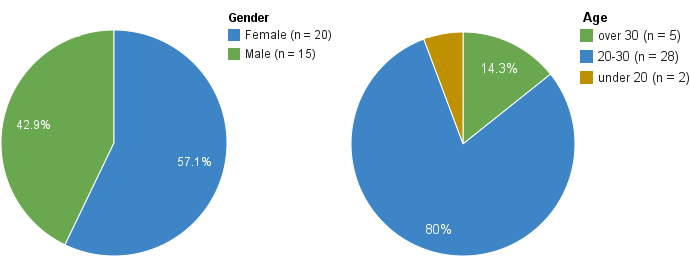
\includegraphics[width=1\textwidth]{CH7-F5-Demographics}
\caption{Participant demographics (n = 35)}
\label{fig:demograph}
\end{figure}

Twenty seven students reported that they were familiar with the concepts
of \LLLs before the experiment. However, only thirteen of these twenty seven
students said that they were familiar with the term \textit{graduate
attributes}. They were primarily Teaching Diploma students. As it was discovered
in informal post-experiment discussion, this might be explained by the fact that
College of Education of Massey University uses term \textit{teaching profile}
instead of \textit{graduate attributes} to describe \LLLs skills and
competences of the degree program.

In the background section, twenty nine students said that they knew about
\textit{\ep} prior to the experiment. Seven of these students reported using an
\ep~system to demonstrate their \LLLsn. They were Veterinary Science students
who had \ep~work included into their degree program curriculum.

\subsection{Activities and Artifacts}

Figure \ref{fig:procedure} provides an overview of the experiment procedure and
the activities or tasks performed for each part, based on the study protocol.

\begin{figure}[htb]
\centering
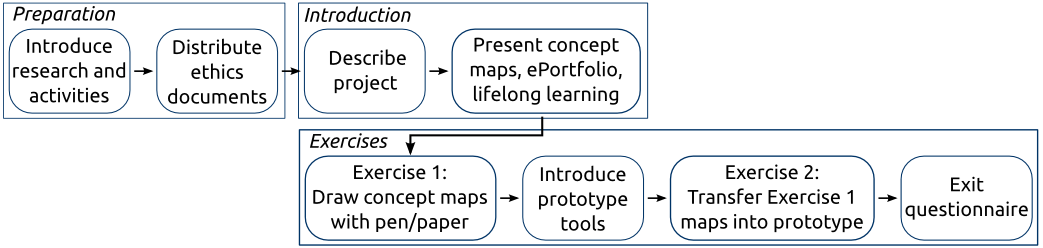
\includegraphics[width=1\textwidth]{CH7-F8-Activities}
\caption{Experiment procedure}
\label{fig:procedure}
\end{figure}

Length of the presentations and information content of the introduction part
varied depending on the participants' experience.

List of the artifacts used by the students in this experiment was following:

\begin{itemize}
  \item Ethics documents: a) information sheet, and b) consent form;
  \item Pen and paper for the first concept mapping exercise;
  \item Examples of the institutional graduate attributes and courses learning
  objectives taken from the Massey University web-site;
  \item Examples of concept maps in the \ep~system created by the researcher;
  \item Instruction sheet with the unique access account to the \ep~system;
  \item User manual for the \ep~system concept mapping tool;
  \item User manual for artifacts fragments extraction;
  \item The exit questionnaire.
\end{itemize} 

Appendix \ref{cha:app6} provides samples of the documents used in the
experiment. Participants' responses from the exit questionnaire can be found in
Section \ref{sec:responses} of this appendix.

\subsection{Data Analysis and Results}

The data collected during this evaluation were based on exit questionnaire
results, observations and system records. These are described in the related
subsections of this section.

\subsubsection{Observed Behaviour}

Based on observations, the most difficult for students was the very beginning of
each of the exercises. In the informal discussion after the experiment, some
of the students admitted that having a blank sheet of paper or an empty
\ep~system account in front of them as they started was rather intimidating. At
first, students expected to be told what to draw and which concepts to include
into their diagrams. After a short explanation that there were no right or wrong
concept maps that could represent their own learning experience or skills, the
process of working with concept maps moved on.

All students were able to complete exercises in allocated time. Students, new to
the concept mapping, followed the techniques presented in the introduction
tutorial on how to build the maps. This included deciding the main message or
the key concept of their map followed by identifying the related concepts. When
this was done, they tried to organize the concepts into maps (Figure
\ref{fig:study2maps}, a).

% TODO: photo of the concept maps on paper
\begin{figure}[htb]
\centering

\includegraphics[width=0.96\textwidth]{CH7-F12-Map-Photo}
\caption{Concept map drawing examples by the students}
\label{fig:study2maps}
\end{figure}

More experienced students preferred to follow their own established procedure of
creating concept maps. Some of them did not spend time making a list of the
concepts, but were adding concepts straight to the maps making corrections when
necessary (Figure \ref{fig:study2maps}, b).

Due to the lack of information about previous experiences of the participants,
in some cases groups consisted of students with very different knowledge of the
discussed concepts. The problem with this situation was that while the students
with no experience required assistance, more experienced participants tended to
jump ahead of the group in doing exercises, following manual on their own and
not waiting for the demonstration of the evaluated functionality of the
prototype. At this stage, it is not possible to analyse whether this had any
influence on the results of the evaluation, as the demonstration which those
students would have followed, had the same information content as the user
manual on the prototype functionality. Therefore, it possible to assume here
that all participants worked under the same conditions.

\subsubsection{Exit Questionnaire Results}
The exit questionnaire responses were the major data collection source for the
user feedback and evaluation.

In general, the responses were very positive. Comments made by the participants
during the exercises showed that they enjoyed the work with concept mapping
tools in the \ep~system.

Based on the responses to the Section B of the exit questionnaire, students
found \ep~concept mapping to be a valuable experience. According to their
comments, the tools and methods that were used during the experiment helped
them to think about bigger picture of their learning, make links between the
concepts they have learnt at the university, think how these concepts contribute
to the skills development, and organize their previous experience in a 
structured way that could be shared with others.

In the informal conversation after the experiment, a number of students asked
for permission to keep the \ep~system login information they have been provided
with for the time of the study in order to use it later on their own. Although,
these students have not been rejected in the system access, they were warned
that the \ep~system prototype was going to be fully supported only for the
duration of the research project. From the perspective of the research
evaluation, this expression of interest can be considered an additional measure
of success of the tools used by the students.

Table \ref{tab:study2summary} summarizes the overall participants experience of
using concept mapping in the \ep~system. The number in brackets indicates the
number of participants who mentioned these features in their responses. In
some cases one student could name more that one feature they liked or not
mention anything at all.

\begin{table}[htb] \small
  \begin{center}
    \begin{tabular}{| p{6.5cm} | p{6.5cm} |}
    \hline
     \multicolumn{1}{|c|}{\textbf{Most favoured part/feature}} &
     \multicolumn{1}{c|}{\textbf{Least favoured part/feature}} \\
     \hline
     Ease of use (11) & Complicated to add examples (6) \\ \hline
     Extracting fragments (7) & Might be time consuming (6) \\ \hline
     Visual representation of knowledge (7) & Might be difficult without initial help (4) \\ \hline
     Link between concepts and experience (5) & Restricted maps formatting (2) \\ \hline 
     Sharing of development (4) & Restricted examples format (1) \\ \hline
     Tracking progress (4) & Learning system is complex (1) \\ \hline
     Shows bigger picture (3) &  \\ \hline
     Targeted reflection (2) & \\ \hline
     Gets the thinking process going (1) & \\ \hline
    \end{tabular}
  \end{center}
  \caption{Participants' feedback on the concept mapping in the \ep~system }
  \label{tab:study2summary}
\end{table}

Examples of responses to the Section B of the exit questionnaire can be found in
Section \ref{sec:responses} of Appendix \ref{cha:app6}.

At the end of the exit questionnaire, the participants were asked to evaluate
usefulness of the used tools based on ten point scale where ten points
represented \textit{highly useful} score and one point represented \textit{not
useful at all} score. Chart \ref{fig:overall} shows the overall scores based on
participants responses.

\begin{figure}[htb]
\centering
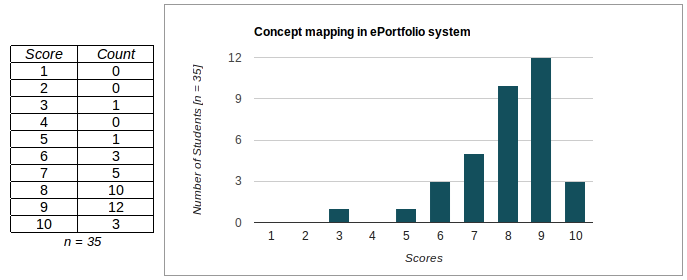
\includegraphics[width=1\textwidth]{CH7-F1-Chart}
\caption{Overall views on usefulness of the used tools and methods}
\label{fig:overall}
\end{figure}

The questions that can be asked here is whether participants' previous
experience with either \ep s systems or familiarity with the \LLLs concepts
influenced the perception of usefulness of the concept mapping tool as a part of
the \ep~system.

For this purpose, the results were split into three groups (Figure
\ref{fig:groups}) based on the differences in participants' experience
reported in the background section (Section A) of the exit questionnaire:

\begin{figure}[htb]
\centering
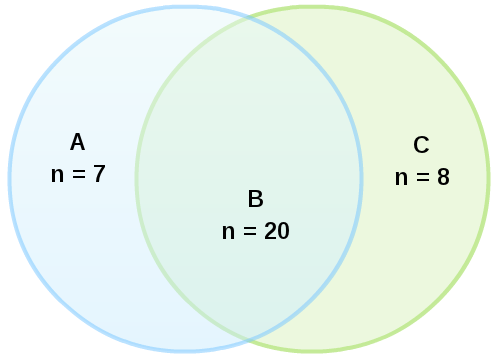
\includegraphics[width=0.5\textwidth]{CH7-F6-Groups}
\caption{Experiment groups based on student profiles}
\label{fig:groups}
\end{figure}

\FloatBarrier

\textit{Group A} represents participants who were familiar with the concepts of
\LLLs prior to the experiment. \textit{Group C} consists of students who have
not been using any kind of \ep~system to demonstrate their \LLLs prior to the
experiment. \textit{Group B} represents an intersection of groups A and C and
therefore consists of students familiar with \LLLsn, but who have not been using
\ep~systems. In this case, \textit{Group A} also represents students who
have used an \ep~system for \LLLs purposes prior to the experiment. Variable
\textit{n} represents a number of participants in each group respectively.

According to such distribution of the participants into groups, the views on
usefulness of the \ep~system concept mapping tools were following:

\begin{figure}[htb]
\centering
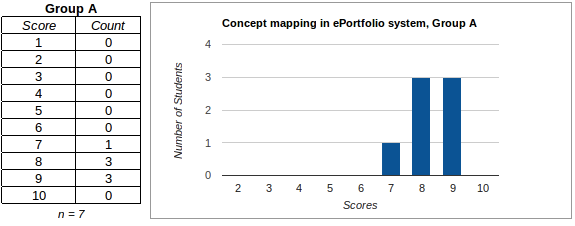
\includegraphics[width=1\textwidth]{CH7-F2-Chart-GA}
\caption{Group A views on usefulness of the used tools and methods}
\label{fig:group1}
\end{figure}

\begin{figure}[htb]
\centering
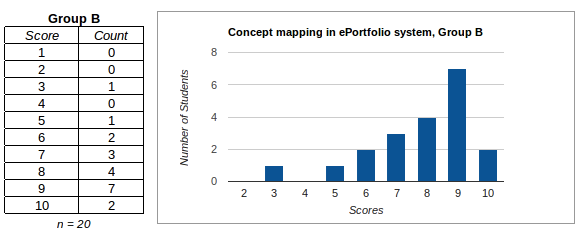
\includegraphics[width=1\textwidth]{CH7-F3-Chart-GB}
\caption{Group B views on usefulness of the used tools and methods}
\label{fig:group2}
\end{figure}

The student from Group B (Figure \ref{fig:group2}) who gave three points to the
usefulness score of the used tools decided not to justify their choice by the
exit questionnaire responses. The only comment they left was \textit{``You can't
quite do what you want with it''} without an overall experience description,
recommended improvements, or description of the least favoured parts.

\begin{figure}[htb]
\centering
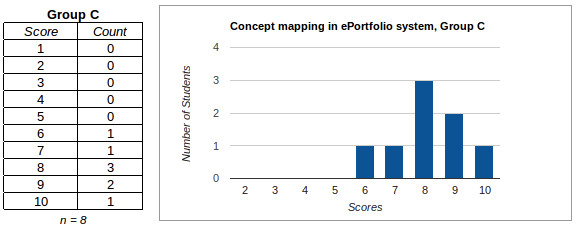
\includegraphics[width=1\textwidth]{CH7-F4-Chart-GC}
\caption{Group C views on usefulness of the used tools and methods}
\label{fig:group3}
\end{figure}

\FloatBarrier

In general, it can be seen that participants of all groups gave high scores as a
measure of usefulness of the concept mapping tools in the \ep~system they had
used. It can be also concluded that the previous experience with the overall
concepts did not have substantial influence on the score distribution. However,
it must be noticed that Group B (Figure \ref{fig:group2}) has a significantly
larger number of students compared to Groups A (Figure \ref{fig:group1}) and C
(Figure \ref{fig:group3}). Nevertheless, the conclusion drawn from this analysis
can be that the novice users find the tools that had been used during the
experiment the same useful as the students familiar with either one or both
concepts of \LLLs and \ep s.

\subsubsection{Concept Maps Created by Students in the \ep~System}

Section \ref{sec:examples1} of Appendix \ref{cha:app6} provides examples of the
concept maps created by the students using \ep~tools during the experiment. As
it was requested by the exercise task, the majority of students transferred
their hand drawn concept maps to the \ep~system prototype. A small number of
concepts had examples attached to them that would demonstrate students'
experience of the related concepts. Due to the fact that the participants had
not been expected to bring examples with them to the study, they were asked to
think about what examples they would include and create empty files or short
blog posts for these. As it was explained to the students, understanding and
evaluation of the general concept rather than content they create was in focus
of this study.

\subsection{Conclusions}

Overall, it can be concluded that the fundamental goal of this study to
evaluate whether the students find prototype tools helpful was accomplished. It
showed that students perception of the concept mapping as a part of the
\ep~system was positive and it provided a suitable means of addressing graduate
attributes and \LLLs skills.

Students who have had prior experience with using the \ep~system to demonstrate
their \LLLs skills said that concept mapping was a great idea and worked better
for them than the \ep~tools they had used before.

Although, usability was not in focus of the prototype requirements, a large
number of students noticed that concept mapping was easy and straightforward to
use. In contrast, extracting fragments of the artifacts and adding them as
examples to the concepts was more complicated and less intuitive task and
required detailed instructions. However, a common agreement among the
participants was that with proper training and experience all tasks can be
easily performed on daily basis.

A problem with the participants testing software rather than evaluating the
overall method and its concepts was expected to be a potential threat to
validity of the outcomes of this study. For this reason, in the introduction
part of the experiment it was emphasized that the participants were going to use
prototype version of functionality and therefore should not pay attention to
the flaws of the user interface, but focus on the process and an overall idea.
Unfortunately, it was impossible to avoid the responses that indicated that
participants were looking at the software and its functionality instead trying
to understand what stands behind it. This could be seen in such comments like
\textit{``Date format on the page is not right for New Zealand''}, \textit{``I
would like to have a choice of color boxes''}, or \textit{``Bigger, more
approachable toolbar would be nice''}. However, there were no more than four
responses similar to these for each question. These responses can be considered
useful in further improvements of the prototype features user interface.

Among the improvements suggested by the participants were:

\begin{itemize}
  \item Simplification of the process of linking examples to the concepts;
  \item Improved maps formatting and reorganizing options for higher
  flexibility of the concepts and better delivery of owners message;
  \item Video tutorial and more detailed instructions on using concept mapping
  tools to ensure that even novice users can start on their own without external
  help;
  \item Options of linking items outside of the \ep~repository to bring other
  sources of learning to the \ep~system;
  \item More examples of the concept maps for students with various profiles --
  resembles the need of providing the students with a model \ep~example.
\end{itemize}

These recommendations can be used to design further improvements to the process
and the overall concept to ensure that they are accepted by the students with
diverse level of experience.
 
\section{Study Three. System Validation by Experienced Students}
\label{sec:three}

The third study in the series of evaluation studies for this research project
investigates whether the prototype features can be successfully employed by the
mature students to provide support for their \LLLs while not being guided by the
lecturer or institutional requirements. This evaluation consists of a series of
case studies which explore the processes and methods used in the \ep~system
prototype with postgraduate students to determine their opinion.

Case studies are commonly used as evaluation method \citep{Yin2012}. The role of
a \textit{case} in the classic case studies is usually played by individuals
\citep{Yin2009}. However, the unit of analysis can be any entity other than a
single individual: case studies can be done about events, programs, processes,
organizations, etc \citep{Yin2009,Patton2002}. The unit of analysis for these
case studies was a prototype of the \ep~system that provided support for \LLLs
in universities.

\subsection{Goals}

The goal for this study was:

\shortquote{To investigate how new features can help students track their
learning progress, manage \ep~knowledge and content, demonstrate and share their
achievements with others.}

To support achievement of this goal, the main objectives were:

\begin{itemize}
  \item To investigate how useful the students find the prototype features for
  the purposes they have been created for;
  \item To explore what are advantages and disadvantages of the implementations
  compared to the other \ep~features which the students have used before;
  \item To demonstrate how the new features can be used by the students for:
  \begin{itemize}
    \item developing understanding of their personal and professional 
    development;
    \item effectively managing their \ep~knowledge and content;
    \item sharing their achievements with others;
    \item communication and getting feedback;
    \item tracking own learning progress; 
  \end{itemize}
\end{itemize}

\subsection{The Case Studies and Participants Profile}

This study was of exploratory nature and used a multiple case study approach as
an instrument of the evaluation. Although, case studies are known for their poor
generalisation (external validity) \citep{Stake1995}, this problem can be
addressed using the strategies described further in this section.

People, places and times are identified by \citet{Trochim2001} as three major
threats to external validity. To overcome these threats and improve external
validity, he suggests to do the study in \textit{a variety of places, with
different people, and at different times} [p.~43]. Due to the unit of analysis
being a prototype system, place for the case studies in this research was not
relevant. 

On the other hand, time of the case studies would potentially matter as each of
the participants was a student and therefore might have depended on the
university semester schedule. In case of Study Three, all participants were
postgraduate students who had their own research project schedule independent of
the university semester. Therefore, due to no major schedule constraints for
participating in this study, time of conducting the study was considered not
relevant as well. 

This study used a mixture of sampling methods to identify the suitable
participants. First, a criterion sampling method was applied which identified
potential cases who met the general criteria of being a postgraduate mature
student and being familiar with the concepts of \LLLs and \ep.

Then, a \textit{maximum variation (heterogeneity) cases} strategy of purposeful
sampling \citep{Flyvbjerg2006,Patton2002} was applied to narrow down the sample
to three cases. According to this strategy, cases have to be different in at
least one dimension (e.g., experience with using \ep~system, participant's age,
area or program of study) to gather information about influence of various
circumstances on processes and outcomes of the case study. This strategy also
follows the recommendation of \citet{Stake1995} according to which researchers
should try to keep balance between the uniqueness and the ordinariness in the
process of case selection.

In summary, the three case studies were carried out with the mature students who
varied in the areas of study and had different experience of using \ep~systems.

\begin{table}[htb] \small
\begin{center}
	\begin{tabular} {| p{3.5cm} | c | c | c |}
	 \hline
	 \multicolumn{1}{|c|}{\textbf{Characteristics}} &
     \multicolumn{1}{c|}{\textbf{Participant One}} & 
     \multicolumn{1}{c|}{\textbf{Participant Two}} & 
     \multicolumn{1}{c|}{\textbf{Participant Three}} \\ \hline
	    Native English speaker & yes & yes & no \\ \hline
	    Age & over 30 & 20-30 & over 30 \\ \hline
	    Degree of study & Masters & PhD & PhD \\ \hline
	    Area of study & Arts & Computer Science & Education \\ \hline
	    Aware of \LLLs & yes & yes & yes \\ \hline
	    Self-rated \ep~use experience (1-10) & 8 & 6 & 8 \\ \hline
	    \multirow{3}{4cm}{Specialized \ep~systems used before}  & 
	    \multirow{3}{*}{MyPortfolio} & \multirow{3}{*}{OSP}  & OSP \\ 
	    & & & The Johns Hopkins DP \\ \hline 
	    \multirow{4}{4cm}{Purpose of previous \ep~use} & Assessment & Research
	    project & Personal development \\ 
	    & C.V. & C.V. & Research project \\ 
	    & Repository & Personal progress & \\
	    & Teaching Aid & & \\ \hline 
	    Currently maintaining \ep & yes & yes & no, but would like to \\
	    \hline
	\end{tabular}
\end{center}
\caption{Study Three participants profile (n = 3)}
\label{tab:study3part}
\end{table}

Table \ref{tab:study3part} shows the background characteristics of the three
participants. As it can be seen, together these characteristics were different
from each other enough to address the issues of poor generalization property of
the case studies as recommended by \citet{Flyvbjerg2006}. At the time of the
evaluation, all three participants were pursuing postgraduate study degrees in
various areas. Apart from being familiar with the \LLLs concepts, this was the
only common characteristics between all three participants.

A self-rated experience of using \ep~systems was relatively similar through all
cases with two participants rating themselves as experienced and one rating as
above average based on scale from one to ten.

Participant One had the longest experience of continually using \ep~system for
various purposes: evidence of personal and professional development, repository
of artifacts, and assessment. As well, they had experience of training others to
use the \ep~system to demonstrate their professional development. At the time of
study, Participant One reported maintaining both personal and professional \ep.

Participant Two with above average experience of using the \ep~systems reported
that they had started using a specialized \ep~system a while back before the
study, but due to personal preferences had returned to their own ways of 
maintaining \ep~through the personal web-site. According to their opinion, this
option provided them with more flexibility and independence from the
institutionally supported, but also limited environments.

Participant Three, while having been actively involved with the \ep~systems
development in their past research carrier, was not maintaining personal \ep~at
the time of evaluation due to the lack of time. As they explained during the
discussion, it was also partly because they could not find a suitable \ep~system
which would provide high-quality free services.

\subsection{Research Protocol}

The study was split into two sessions held in separate meetings with each of
the participants. The main strategy for this study was to give the participants
access to the \ep~prototype environment for a certain period of time so that
they could try the new features on their own and in their own time.

The first session was an introductory meeting and was conducted to familiarize
the participants with the environment they were going to evaluate. Before
starting any study activity, each participant was provided with the information
sheet which stated their rights and the consent form to sign in case they agree
to participate under the conditions outlined in the information sheet. None of
the students had objections to the study conditions.

After all ethics arrangements were finished, the researcher gave a brief
presentation on the research project and the aim of the study. Participants were
demonstrated each implemented feature that was in focus of the evaluation,
explained its purpose and given the examples of potential use. Unlike in the
experiment of the Study Two, in this study, the participants did not have
exercises to complete or tasks to follow. Instead, they were given freedom to
choose what activities to perform given a set of prototype features to evaluate.
Each of the students had an access to the user manual for the features they were
trying out. 

For the evaluation time, the \ep~system prototype was available 24 hours a day
and could be accessed from outside of the university network. This was done so
that the students could work with the system from home and did not depend on
being in the university. To access the features of the system, each student had
to create their personal account which they had to use till the end of the
evaluation period.

All participants were told that the researcher would regularly check on their
progress. As well, they were suggested to contact the researcher any time they
required assistance or when they were ready to discuss the implementations they
had used.

All students were given time to work with the \ep~system prototype until the end
of the calendar year when the evaluation stage was scheduled to finish. This
arrangement would have given each of the participants on average four months of
trial period. Participants Two and Three contacted the researched in less than
one months to schedule the second meeting. Participant One took one and a half
months get back to the researcher with their feedback.

The second session was a discussion meeting organized with each of the
participants after they had finished their evaluations of the prototype. During
the meeting they discussed the ways they employed the new features and how
helpful these features were for the purpose. One of the participants showed
what they had done and during the demonstration pointed out the problems they
had while working with the system. Where possible, each student was asked to
describe advantages and disadvantages of the new features compared to the
\ep~features they had used before. Lastly, they were offered to recommend any
future improvements.

Discussion with each participant took on average 90 minutes and was audio
recorded for the purposes of transcribing and analysis. At the end of the
meeting, the participants were asked to complete a background questionnaire and
provide any other comments that might be valuable for the research evaluations.

According to the participants' requests, they retained their access to the
prototype system after the meeting for the duration of this research project.

The research protocol, examples of potential questions for the discussions, the
background questionnaire, and all other documents related to the Study Three can
be found in Appendix \ref{cha:app7}.

\subsection{Data Analysis and Results}

Each of the case studies utilized multiple sources for data collection:
background questionnaires, semi-structured as well informal discussions, records
made by the participants in the \ep~system, uploaded artifacts, and system logs.

While the participants had access to the evaluated \ep~system, it was possible
to track their system usage: how many times they logged into the system, what
resources they uploaded, and what kind of records they created. However, this
information did not provide the evidence of how long was spent by each of the
participants working with the evaluated features. In this case, the researcher
had to rely on what the participants said at the second meeting.

Based on the system logs, Table \ref{tab:study3stats} shows statistics of the
\ep~system usage by the participants:

\begin{table}[htb] \small
\begin{center}
	\begin{tabular} {| p{3.5cm} | c | c | c |}
	 \hline
	 \multicolumn{1}{|c|}{} &
     \multicolumn{1}{c|}{\textbf{Participant One}} & 
     \multicolumn{1}{c|}{\textbf{Participant Two}} & 
     \multicolumn{1}{c|}{\textbf{Participant Three}} \\ \hline
	    Length of access\footnotemark[1] & 37 days & 7 days & 15 days \\ \hline 
	    No. of logins & 4 & 6 & 5 \\ \hline 
	    No. of records created & 29 & 58 & 23 \\ \hline
	    No. of files uploaded & 8 & 6 & 4 \\ \hline
	\end{tabular}
\end{center}
\caption{The prototype usage statistics}
\label{tab:study3stats}
\end{table}
\footnotetext[1]{Calculated based on the difference between account registration
date and last access date}

During the second session, the researcher discussed system usage log information
with the participants. According on their opinion, all participants considered
that they had had sufficient time to explore the features. 

In general, according to their feedback, all participants viewed the prototype
implementations positively. At the end of the meeting, one of the students said:
\textit{``I've seen a lot of interesting ideas in this system and I would like
to see them moving to the new version of the \ep~system.''}. This can be
interpreted as one of the indicators of success of the \ep~system prototype with
the representatives of the mature student audience.

To take a closer look at the results of the evaluations, each feature is
described further in this section as it was discussed with the students during
the meeting. Direct quotes were taken from the audio recordings transcripts.
Examples of the features usage are the snapshots from the students' system
account.

\subsubsection{Concept Mapping Module}

Participant One called the concept map module as \textit{a really good visual
way to navigate around the entire \ep.}

Figure \ref{fig:p1map} shows a simple concept map created by Participant One in
order to try out the feature:

\begin{figure}[htb]
\centering
\setlength\fboxsep{0pt}
\setlength\fboxrule{0.5pt}
\fbox{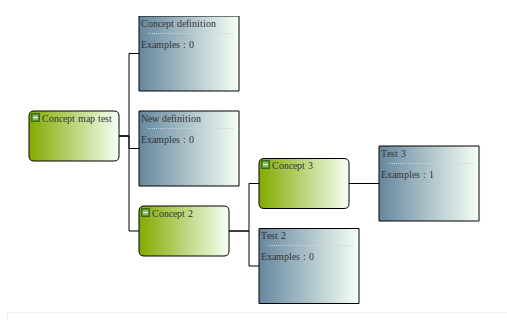
\includegraphics[width=0.7\textwidth]{CH7-F10-Example2}}
\caption{A concept map created by Participant One}
\label{fig:p1map}
\end{figure}

One of the drawbacks of concept mapping as described by Participant One was
that they found it difficult or almost impossible to make complex concept maps.
However, this limitation was due to the prototype level of implementations
rather than shortcomings of the underlying concept. Participant One liked the
idea of concept mapping as a part of the \ep~system. Although, they said that it
should be expected that, as the users become more confident with the system,
they would want to build more complex links between concepts which is not
possible at the moment.

Participant One admitted that they used the concept mapping feature and other
features that were connected to it more than they used anything else in the
prototype. They considered the idea of using concept maps for content and
knowledge management as very promising, but it should be taken to another more
complex level:

\shortquote{Participant One: An interesting idea would be to to be able to
aggregate anything that is added to \ep~by\ldots let's say, tags. For example, I
tag the blog post with this concept tag, and next time I open concept map, I can
see it linked to that concept. I really would like the concept maps to
practically build themselves.}

When the researcher noticed that in this case the idea of meaningful linking of
items in the \ep~system might be lost, Participant One agreed that there should
be a balance between the things that are done automatically and the things that
user would have to do manually.

\begin{figure}[htb]
\centering
\setlength\fboxsep{0pt}
\setlength\fboxrule{0.5pt}
\fbox{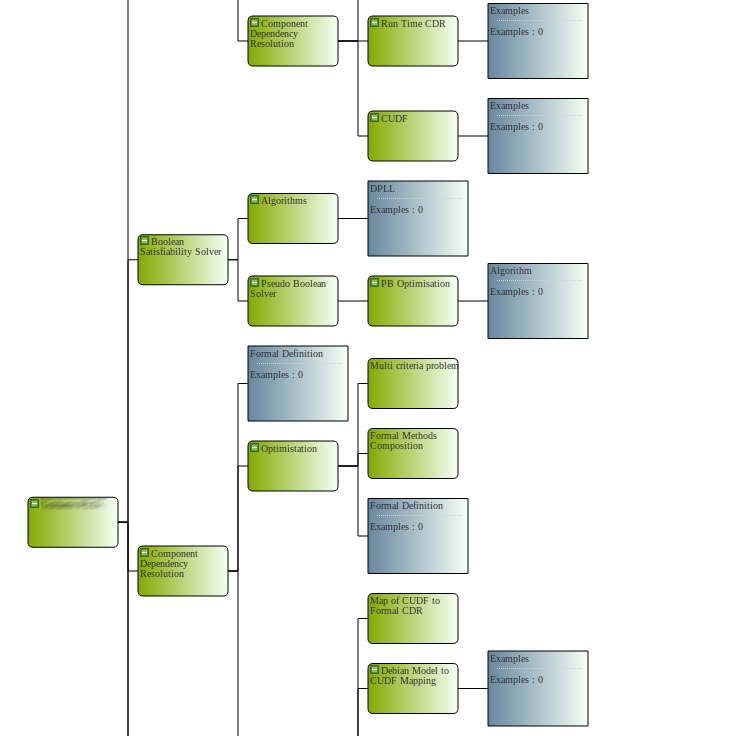
\includegraphics[width=0.9\textwidth]{CH7-F9-Example1}}
\caption{A fragment of a complex concept map created by Participant Two}
\label{fig:p2map}
\end{figure}

As shown on Figure \ref{fig:p2map}, Participant Two used concept mapping to
organize knowledge accumulated and concepts learnt during their PhD studies.
They said that using the tool for this purpose helped them to understand what
has been already done and what would still have to be done in the future.

Participant Two who had prior experience of using rubrics matrix in another
\ep~system as a way of addressing \LLLs skills said that they found the concept
mapping in this \ep~system as much more intuitive knowledge visualization tool
and a tool for demonstration of understanding and achieving objectives.

Participant Two said that \ep~concept mapping was an \textit{excellent tool},
though it required some further improvements of visual personalization. The main
benefit of the feature for Participant Two was in organising and connecting the
various threads that had been learnt. 

\shortquote{Participant Two: It helps to organise and also display the current
progress and review different ideas easily. I feel if the graduate attributes
were there and the students gave examples of these attributes, it would make it
easier to see why certain things were learnt.}

Participant Three found that the idea of adding concept maps to the \ep~system
was \textit{very nice}. They had the long-term prior experience of using concept
mapping technique as a teaching aid at school. Participant Three thought that
linking concepts was particularly good principle in \ep~when learners could
create connection between things they had done.

Participant Three also said that concept maps were user-friendly and their
layout was as well easy for reading. However, similarly to Participant Two, they
suggested that concept maps need more formatting options. While it was not a
major improvement, it would add another level of personalization:

\shortquote{Participant Three: There is a lot of visual learning going on
nowadays. Different learners have different ways of seeing things and being able
to change\ldots shape things according to their views is important if we want to
have an \ep~that is really personal.}

Among the suggestions for improvements to formatting of the concept maps
named by Participant Three were:
\begin{itemize}
  \item Adding labels to the links between concepts;
  \item Color choice for concepts;
  \item Change of orientation of the maps;
  \item Concepts sorting within the maps;
  \item Reorganizing the concepts inside the map.
\end{itemize}

To justify these suggestions, Participant Three explained:

\shortquote{Participant Three: Although, I think the best way to read maps is
when they are laid out like in the prototype, sometimes people just want to try
out how it would look like another way. It might be useful to have an option of
organizing concepts in the maps in their own way.}

Participant Three did not to provide their examples of concept maps.

Overall, from the feedback given by all participants it can be concluded that
concept mapping as a part of the \ep~system was accepted as a valuable tool to
organizing \ep~knowledge, navigating through the \ep~concepts, demonstrating
achievements of learning objectives, and evaluating of personal learning
progress.

\subsubsection{Artifacts' Fragments Extraction}

Being an Art's student highly involved in design and visual arts, Participant
One was particularly interested in this feature. They said that it would be an
easy way of emphasizing fragments of a visual work and drawing attention of
others to the particular elements of the displayed artifact.

\shortquote{Participant One: The idea of fragments is really interesting. I
haven't seen it in the \ep~systems before.}

Participant Two liked the idea of fragments in terms of viewing a single
document from different perspectives to see what concepts had been learnt. They
said that this feature could be used for splitting up artifacts into different
examples to be presented in the concept map.

From the perspective of their professional field, Participant Two understood the
difficulties of marking up or selecting fragments of the documents that had
proprietary format. However, they said that there could be an choice for users
to open a document as a plain text file for fragment selection. Users generally
know whether their document can be opened in plan text format. This would be
very useful for the students in technical areas, such as Participant's Two,
where a lot of skills are demonstrated in programming and code samples.

Participant Three said that fragments of the artifacts might have a potential
value of communicating ideas more clearly between a learner and a teacher.
From this perspective, selecting an exact part of a picture or limiting a long
video to just a number of time frames allows to be more specific about the
things that students might want to share.

Compared to other \ep~systems, Participant Three liked that reflection could be
directly attached to a potential evidence of any concept from a concept map.
They said that it should be useful for students to be able to explain what and
why they added to their \ep.

It can be concluded that all three participants understood the general principle
of working with this feature. Each of them saw the various ways of applying it
together with the other prototype features in the \ep~system for better
reflection, sharing and emphasizing elements of one's learning that contribute
to the bigger picture of personal development.

\subsubsection{Learning Progress Tracking}

Each of the participants had a common view that timeline-based progress tracking
feature was useful for discovering gaps in their learning and demonstrating
improvements towards achievement of their learning goals. For example,
Participant one said:

\shortquote{Participant One: The timeline is really useful actually in the way
that I can get a really quick look at my progress and re-factor my gaps.}

\begin{figure}[htb]
\centering
\setlength\fboxsep{0pt}
\setlength\fboxrule{0.5pt}
\fbox{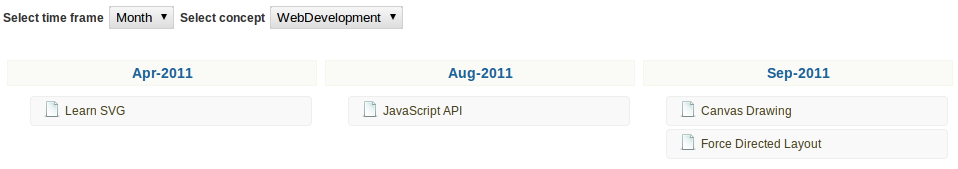
\includegraphics[width=1\textwidth]{CH7-F11-Example3}}
\caption{Progress tracking example by Participant Two}
\label{fig:p2timeline}
\end{figure}

Figure \ref{fig:p2timeline} shows one of the examples of using progress tracking
feature provided by Participant Two. According to them, the timeline
functionality was an \textit{excellent way of viewing progress} which allowed to
see achievements of the past and learning potential for the future:

\shortquote{Participant Two: It enables the view of what I have done and then I
can also see areas for improvement.}

Participant Two did not like the way custom time-frames were supposed to be
created by the users. They found the implementations to be confusing and not
straightforward, although the overall idea looked interesting to them. They
suggested that this part would either require more detailed explanation to the
learners who are just starting to use the \ep~system or considerable changes to
the way custom timelines and time-frames are created.

Participant Three thought that together with the concept mapping tools timeline
provided another perspective on learning. According to their opinion, if used
properly, these features could be a very powerful tool for lecturers to perform
assessment.

\shortquote{Participant Three: In the concept map, someone can see how I
understand the knowledge concepts, while in timeline I can easily show what I
have actually done to address these concepts [\ldots] If I was teaching now, I
would definitely use it with my students.}

Participant One noticed that this feature did not require any manual input from
the users. Although, timeline representation builds itself from the concepts and
examples that learners provide in adjacent features, there might be a room for
data manipulation on timeline level as well. For example, students should be
able to drag examples between time frames which would allow them to easily
update date of an example. Another potential improvements would be a color
highlight of the elements on timeline based on the examples association with a
concept.

Overall, all participants were satisfied with the feature and said that they
could see it working for the purpose of learning progress tracking for students
as well as for lecturers.

\subsubsection{Version Control Elements}

Version control feature was implemented through a simple page versioning in the
\ep~repository. Participant Two really liked the idea of adding this kind of
functionality to the \ep~system.

\shortquote{Participant Two: Everything in \ep~should be done with versions. It
might be my Computer Science background, but for me it's a really good way of
own seeing progress in work.}

According to Participant's Three views, in addition to being able to show the
changes that had been done in the process of developing a showcase \ep~page,
this feature would also help to support discussion between a learner and other
interested parties. An opportunity to justify the changes and communicate the
improvements is a valuable addition to the conventional \ep~systems'
functionality.

\shortquote{Participant Three: I think adding version control elements to the
\ep~system is an excellent idea. It would be useful in many circumstances to
view changes and improvement.}

Participant One said that in the way it is implemented now, \textit{the
lecturers might enjoy this feature much more than students}. As they explained,
traditionally version control features were used for an opportunity to go
back and revert the changes rather than review the progress made between
versions. In case of this implementation, it was more like a version release of
a software when one can introduce improvements and share them with others.
Participant One could not imagine going back and trying to compare versions of
pages, but from the perspective of a lecture, their dialog with a student
that could be supported this way, and an opportunity to review students'
progress, it seemed to be useful.

It can be concluded that all three participants found this feature useful for
the purpose it was created. None of the students could not think of any other
potential applications than the ones suggested by the researcher.

\subsubsection{Shared Resources Management}

Due to the system being a prototype with no social activity going on, none of
the participants could properly test the all features implemented for the shared
resources management. Participant One found the way out by registering another
account and sharing resources between the two accounts. Other participants
followed the descriptions in the user manual and looked at the feature's set ups
without actually sharing resources with anyone. In some cases, they tried out
giving feedback to their own artifacts and other items, or sharing resourced
with the friends group and logged-in users.

Participant Two said that it might be difficult to measure the effectiveness
of the shared items management by just sharing something with others or
compiling a C.V. for a potential employer. According to their point of view, the
problem with this approach would be that there were already effective mechanisms
in place that allowed sharing resources. However, the valuable benefit of this
feature in the \ep~system prototype would potentially be in combination with the
version control feature in order to manage changes and feedback to the artifacts
at the same time.

Participant One noticed that notifications about access to the shared resources
in the \ep~system might not be positively accepted by some users. From the
perspective of people outside of the \ep~community, such notifications might
turn the \ep~system into another spam sending web-site. From their point of
view, this feature required much more options to consider for both a sender and
a person who would receive notifications.

Although, none of the students could evaluate full potential of this feature,
they all said that they could see it being helpful combined with other features
for \LLLs support. However, from the research perspective, these assumptions
have to be tested by further investigations.

\subsection{Conclusions}

Overall, based on the evidence gathered during the case studies, it can be
concluded that all three participants supported the prototype implementations
and agreed that being properly utilized these implementations could be a part of
a successful approach to \LLLs support in universities.

Although, all three participants were generally satisfied with the
implementations, they also tended to suggest a number of improvements for each
feature. These included the following:

\begin{itemize}
  \item improvements to the concept mapping tool for better interaction,
  flexibility and user control;
  \item improvements to the artifacts' fragment extraction to provide users with
  more file options and better communicating their ideas;
  \item improvements to the shared resources management with more opportunities
  for a sender as well as a recipient; 
  \item improvements to the progress tracking using more intuitive creating of
  custom timeline and time-frames;
  \item improvements to the version control feature with more \ep~artifacts
  having version property.
\end{itemize}

Due to some of the tested features' dependence on the social interactions
between the users, it was not possible to evaluate the entire prototype in depth
as it would be necessary before launching the system into the real world
settings. Evaluation according to the thoroughly designed scenarios of potential
use with a larger number of participants would decide strengths and weaknesses
of the implementations performance and feasibility of their use in the social
settings. This can be one of the questions for the future research.

\section{Summary}

This section presented the evaluation design and the results of the evaluation
of this research project's contributions. Three studies were carried out to
understand how the new features can be utilized by the stakeholders to provide
better support for \LLLs in the universities.

The results of these studies can be summarized as follows:

\begin{enumerate}
  \item Lecturers see the ways and are willing to incorporate the new features
  into their teaching to provide students with their guidance and help them to
  understand \LLLs skills.
  \item Based on the experiment results, concept mapping as a part of the
  \ep~system can be successfully used by students to demonstrate learning
  achievements and address institutional graduate attributes. It also can
  provide opportunities for targeted reflection and better feedback.
  \item According to the case studies, students see the new features as
  helpful and useful for tracking their learning progress, managing
  \ep~knowledge and content, demonstrating and sharing their achievements with
  others. Further improvements are still required to make the features more
  flexible, intuitive and user-friendly. This would also ensure that the
  evaluation of the underlying concepts have not been affected by the limits of
  implementations.
\end{enumerate} 

An apparent issue of the evaluation was in the fact that it was very difficult
for some of the participants to give their opinion of the underlying concepts
without paying attention to the shortcomings of the user interface. The
evaluated system was a functional prototype and therefore was not aiming at
providing highly attractive and usable user interface. However, this problem
should be considered and addressed in any future research.
